\chapter{Hybrid Neural Network for State Inference} \label{sec:approach}
In this section, I describe my proposed deep learning approach for the black-box state inference task, in details. 

\section{The Model Architecture}
\begin{figure*}
    \centering
    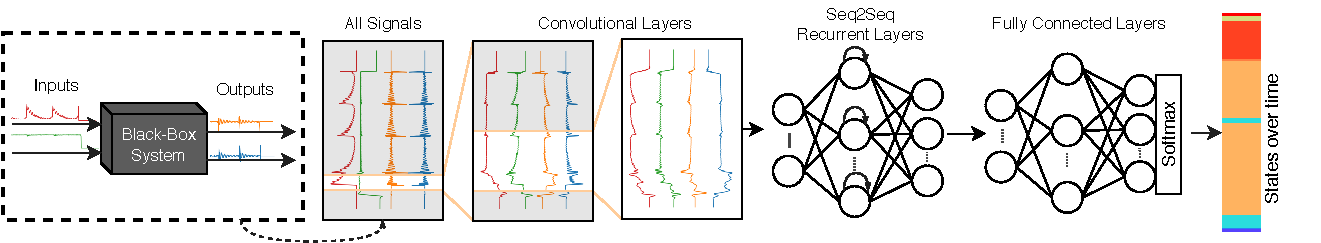
\includegraphics[width=\textwidth]{ASE_files/GeneralConvolutionalNet.pdf}
    \caption{The input and output signals of the black-box system are captured as a multivariate time series; they are processed in a deep neural network that consists of 3 sections: convolutional, recurrent, and dense (fully connected) to predict the system's internal state and its changes over time.}
    \label{fig:general_net}
\end{figure*}

The goal of this study is to infer the states of a running software system, over time. Given that my assumption is we do not have access to the source code (or part of it), I only leverage the values of inputs and outputs of the system, over time.
As can be seen in figure~\ref{fig:general_net}, I capture all the inputs and outputs of the system as a time series and then process it in a DNN. 
The architecture of my proposed model is a hybrid DNN which is inspired by models proposed in the field of Human Activity Recognition (HAR). This task is quite similar to the subject of this thesis in the sense that they both take in a multivariate time series-data (from sensor readings) and output the state of the system that generated those readings (see section~\ref{sec:related_work_har} for more details on HAR papers). 
This DNN is made of three parts in sequence: 1) Convolutional, 2) Recurrent, and 3) Fully connected layers. This architecture addresses the aforementioned traditional methods' challenges; each part serves a different purpose in this process, as follows.


Convolutions, being more generalized than simple sliding windows, can discover patterns and features in the signals, both in temporal and in spatial (how signals affect each other) dimensions \cite{wang2017time}. 
The convolutional layers' flexibility allows them to learn some typical preprocessing operations. For example a moving average or a discrete derivative can be learned as simple convolutional filters. They also help the model to be more resilient to varying time delays between noticing a deviation in input signals and the reaction that will appear in the output signals. Applying convolutional layers in sequence has been shown to result in each layer learning more complex features than the previous layers \cite{zeiler2014visualizing}.
The number of layers, filters, and the kernel size are hyper-parameters that should be selected based on the size of data and the complexity of the system being modeled.
Using a sequence of convolutions with a) increasing number of filters and the same kernel size, b) same number of filters and increasing kernel size, and c) decreasing filters with increasing kernel sizes are all different approaches that have been used in the literature by well-known architectures such as VGG and U-net \cite{simonyan2014very, ronneberger2015u}. 
I will discuss more details of CNN layers in my approach in Section~\ref{sec:architecture_detail}.

Convolutions are quite powerful in discovering local features. To capture long-term features, recurrent layers which learn sequences of data are leveraged. For example, in my case, they can learn that ``accelerate'' and ``take off'' states only happen in the start of the states sequence, and each ``take off'' state is usually followed by a ``climb'' state. The type of recurrent cell to use (LSTM, GRU, etc.), how many cells to unravel in the layer, and the number of layers are also hyper-parameters that need to be tuned depending on the size and complexity of the system under study.

Finally, one or more dense (fully connected) layers in the end are a common way of reducing the dimensions to match expected output dimensions. 
If there are only two states, the last layer can have a sigmoid activation function and be of shape $L$ (the length of the input), otherwise, to match the one-hot encoding of labels, an output of shape $L\times N_s$ with softmax activation along the second axis ($N_s$) is required ($N_s$ being the number of possible states).

In terms of loss function to optimize in the training process, a good choice is a dice overlap loss function, which is used in image semantic segmentation tasks, as well. An important property of this loss function is not getting negatively affected by class imbalances \cite{milletari2016v, sudre2017generalised}.

% To make it more clear, compare it to applying a convolution (or a discrete derivative) to each signal independently. It can only learn temporal features, nothing about the interactions between the signals.
% Using convolutional layers instead of predefined kernels allows the model to learn which subset of possible connections and interactions (which can involve two or more variables) can be used as features. This flexibility has another advantage as well. It helps the model to be more resilient to time lag between noticing a deviation in input signals and the reaction that will appear in the output signals. This time lag can be caused by a number of reasons including: physical limitations, sampling resolution, tuning of the controller, or design choices in the system.
%\subsubsection{Data Collection}
%The object system is treated as a black-box where I can only read its input and output values.
%Capturing the input and output data ($T_k$s) is straightforward. In the first step the system is executed and multiple logs of the input/output values are recorded. After that, state change points ($CP_k$s) data is required to be collected. A typical way to obtain them is with help of a domain expert. They label the logs indicating the time stamps where the system's internal state has changed as well as the new state that it went in. Domain experts are ideal for labeling since they know what the system is and what it is supposed to do, so they can (probably with some inherent human error) detect the system state. 
%They can do it based on a variety of information sources such as examining the system's I/O (which we already have captured), logs, or a high level program or set of instructions preloaded into the system.


%I aimed to infer high level states of a black-box system using a machine learning model that observes the system's behavior.
\section{Data Encoding}
% To collect data I run the system $N$ times using $N$ existing test cases and record the input/output values. The recorded data from $k$-th run, $T_k$, forms a discrete multivariate time series data.
The input/output values of the black-box system create a multivariate time-series ($T_k$), which can be defined as a set of $n$ univariate time series ($V_i$) of the same length $l_k$. Each $V_i$ corresponds to the recorded values for one of the inputs or outputs of the system:
\begin{equation} \label{eq:T_k}
    T_k = \{{V_1}_k, {V_2}_k, \ldots, {V_n}_k\}
\end{equation}
\begin{equation} \label{eq:l_k}
    |{V_1}_k|=|{V_2}_k|=\ldots=|{V_n}_k|=l_k 
\end{equation}

Note that, as figure~\ref{fig:general_net} shows, we take both inputs and outputs as part of the time-series data to be fed as input into my deep learning models.
This is to make sure that we can model state-based behavior of the system, where the current state depends not only on the inputs, but also on the last state(s) (captured as previous outputs) of the system. As an example, from the case study, if the outputs are not taken into account
% the ``acceleration'' state before ``takeoff'' and the breaking state after landing
a mid-flight ``descend'' state and the ``approach'' state right before landing
are indistinguishable, using the sensor readings (inputs) alone. 

Having such a time-series, the only remaining pieces from a training set are the labels. Unlike the input/output values (the features in the data set) the labels are not usually given. My method to infer the labels is a supervised approach. Thus, I need the domain expert to manually label each individual time stamp with a state name/ID. In practice, what they would do is to identify the approximate time that a state change happens and assign the new state to one of the previous states labels or define a new label for this new state.
Thus I encode the states information over time as a set of tuples in the form of $(t_s, s)$ where $t_s$ denotes the timestamp where the system entered state $s$. We show the set of all possible states with $S$ ($s \in S$) and define $N_s$ as the cardinality of this set.
\begin{equation}\label{eq:change_point}\begin{split}
    CP_k {}&{}= \big\{ (t_{s_1}, s_1), (t_{s_2}, s_2), \ldots, (t_{s_l}, s_l) \big\}\:,\; s_i \in S \\
    N_s  {}&{}= |S|
\end{split}
\end{equation}
So in summary, the dataset consists of $N$ pairs of the I/O values as features and their state information as labels $\big\{(X=T_k,\;y=CP_k)|1\leq~k\leq~N\big\}$. 
% Each example in dataset contains one whole test case. The output labels were one-hot encoded to match the model output shape.
%It is worth mentioning that in section~\ref{mp_data_collection} I explain what I did to keep the variety of the collected data (and hence its quality) high.

\subsection{Data Preprocessing}
%\subsubsection{Inputs and Labels} %\label{data_set_properties}
Before being fed into the model $\mathcal{F}$ (as defined below), the inputs and labels need some preprocessing. 
\begin{equation}\label{eq:model_F}
    \mathcal{F}(\delta(T), m) \colon \mathbb{R}^{L\times n}\times\mathbb{R}^L\to S^{L}.
\end{equation}
To run more efficiently, TensorFlow expects all the inputs to have the same length. To do that, the shorter $T_k$s should be zero-padded to length $L = max\{l_k\}$. The padding function $\delta$ does that.
Therefore, eventually, the input to the model will be $T_k$s that are rearranged to form a tensor of shape $n \times L$ along with a padding mask (denoted with $m$). 
The mask tells the model where the tail starts so the model can ignore all the zeros from there on. % It prevents the added zero values to have a negative effect on the model's performance.
%The inputs are the sampled in/out values of the system given in form of $n$ time series of length $L$.
\begin{equation}\label{eq:model_as_function}
\begin{split}
    \hat{O} {}&{}= \langle \hat{o}_i \in S \rangle^L_{i=1} = \mathcal{F}\left(\left[ {\delta(V_1)}^\intercal \: {\delta(V_2)}^\intercal \; \ldots \; {\delta(V_n)}^\intercal \right],m\right) \\
    % \delta(V_i) {}&{}= \left[V_i \quad \vec{0}_{L-l}\right] \\
    m {}&{}= \delta(\vec{\mathds{1}}_l) \quad\text{i.e.}\quad \langle {m}_j \rangle^l_{j=1} = 1\:, \: \langle {m}_j \rangle^L_{j=l+1} = 0 \\
\end{split}
\end{equation}
Here $l$ denotes the length of the input before padding. It is equal to $l_k$ for the $k$th training data ($T_k$).


As defined in \eqref{eq:change_point}, $CP_k$s are tuples of $(t, s)$ which indicate the system have gone into state $s$ at time $t$. To train the model, $CP_k$ needs to be expanded into a vector of length $L$ denoted by $O$ where each element $o_t$ holds the state at time $t$. To define it formally, the elements can be derived from $CP_k$ using the following formula:
\begin{equation} \label{eq:output}
\begin{split}
O = \langle  \forall t \in \mathbb{N}_L : s_i \:|\:
           (& t_{s_i}, s_i) \in CP_k \: \land  \\
            & t_{s_i} = max\{t_{s_j} \:|\: (t_{s_j}, s_j) \in CP_k \land t_{s_j}\leq t\} \rangle
\end{split}
\end{equation}
For example: Suppose $L=10$ and $CP = \{(0, a),\:(3, b),\:(5, c),\:(8, a)\}$ 
% which means starting with state $a$ then going to state $b$ at time $t=3$,\ldots and it goes on for 10 steps; 
then $O = \langle a\:a\:a\:b\:b\:c\:c\:c\:a\:a \rangle$.
If there are more than two possible states ($N_s > 2$), $O$ needs to be one-hot encoded, at this stage.



\section{The Model Implementation} \label{sec:architecture_detail}
The first few layers of the model are convolutional layers. I used 5 convolutional layers with 64 filters each and a growing kernel size.
The intuition behind this design is that starting with a small kernel guides the training in a way that the first layers learn simpler more local features that fits in their window (kernel size).
Kernel sizes started with 3 since it is a common number in the literature for kernel sizes, then I used multiples of 5 from 5 to 20. 
The rationale behind choosing 5 is because the sampling frequency is 5, so each layer with a kernel size of $5n$ processes a whole $n$ seconds worth of simulation data, in each step.
Stopping at kernel size of 20 was a compromise between generalizability and model size. Generally, a larger model has more learning capacity, but it is also more prone to over-fitting. The current models are the smallest I could make the models (to avoid over-fitting), without compromising the performance.

Same compromise was made in the second section of the model (Recurrent layers), the sweet spot for hyper-parameters here was to use two GRU layers with 128 cells each. Their output was fed into a fully connected layer with 128 neurons with a leaky ReLU ($\alpha=0.3$) activation function \cite{maas2013rectifier} and finally to a dense layer with $N_s=25$ units with softmax activation.
I used Adam optimizer \cite{kingma2014adam} that could converge in 60-80 epochs, i.e. validation accuracy plateaued. The full architecture can be seen in figure~\ref{fig:model_arch}.
\begin{figure*}
    \centering
    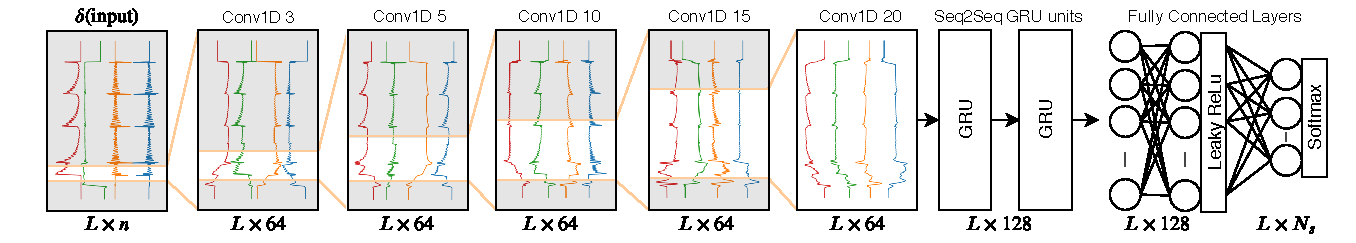
\includegraphics[width=\linewidth]{ASE_files/Convolutional_Net.pdf}
    \caption{Model architecture in a nutshell. Tandem convolutional layers with increasing kernel size fed into two sequence-to-sequence recurrent layers with 128 GRU cells each, which is then fed into dense layers to output the predicted system state, as a list of one-hot encoded states. $\hat{O}$ will be the result of applying argmax operation on the last layer's output. $L=18000,\: N_s=25$}
    \label{fig:model_arch}
\end{figure*}

